\documentclass[usepdftitle=false,hyperref={pdfpagelabels=false}]{beamer}

% use KIT-Theme
% see http://sdqweb.ipd.kit.edu/wiki/Dokumentvorlagen
%\usetheme{Frankfurt} % see http://deic.uab.es/~iblanes/beamer_gallery/index_by_theme.html as fallback
\InputIfFileExists{../templates/beamerthemekit.sty}{\usepackage{../templates/beamerthemekit}}{\usetheme{Frankfurt}}
\usefonttheme{professionalfonts}

\usepackage{hyperref}
\usepackage{lmodern}
\usepackage{listings}
\usepackage{wrapfig}        % see http://en.wikibooks.org/wiki/LaTeX/Floats,_Figures_and_Captions
\usepackage[utf8]{inputenc} % this is needed for german umlauts
\usepackage[ngerman]{babel} % this is needed for german umlauts
\usepackage[T1]{fontenc}    % this is needed for correct output of umlauts in pdf
\usepackage{verbatim}
\usepackage{relsize}
\usepackage{subfigure}
\usepackage{algorithm,algpseudocode}
\usepackage{minted}         % needed for the inclusion of source code
\usepackage{xcolor}
\usepackage{menukeys}
\usepackage{../templates/myStyle}

\newcommand\tutor{Martin Thoma}
\newcommand\tutNR{10}
\newcommand\titleText{Programmieren-Tutorium Nr. \tutNR{} bei \tutor}
\institute{Fakultät für Informatik}

\hypersetup{pdftitle={\titleText}}
\beamertemplatenavigationsymbolsempty

\newcommand\InsertToC[1][]{
  \begin{frame}{Outline}
    \tableofcontents[subsectionstyle=show/show/show, subsubsectionstyle=show/show/show, #1]
  \end{frame}
}

\begin{document}
\title{\titleText}
\subtitle{Eclipse, Arrays, Kontrollstrukturen und Konventionen}
\author{\tutor}
\date{\today}
\subject{Programmieren}

\frame{\titlepage}

\frame{
    \frametitle{Inhaltsverzeichnis}
    \setcounter{tocdepth}{1}
    \tableofcontents
    \setcounter{tocdepth}{2}
}

%\AtBeginSection[]{
%    \InsertToC[sections={\thesection}]  % shows only subsubsections of one subsection
%}

\section{Einleitung}
\subsection{Quiz}
\begin{frame}{Quiz}
    \inputminted[linenos=true, numbersep=5pt, tabsize=4, fontsize=\small]{java}{Quiz.java}
    \begin{itemize}
        \item Was ist die Ausgabe?
        \item Gibt es einen Compiler-Fehler?
        \item Gibt es einen Laufzeit-Fehler?
    \end{itemize}
\end{frame}

\subsection{Quiz: Antwort}
\begin{frame}{Quiz: Antwort}
    Ein Compiler-Fehler:
    \inputminted[linenos=true, numbersep=5pt, tabsize=4, fontsize=\small]{console}{Quiz-Answer.sh-session}
\end{frame}



\section{Eclipse}
\subsection{Frühere Folien}
\begin{frame}{Frühere Folien}
    \begin{itemize}
        \item Installation (für Windows): \href{http://www.eclipse.org/}{eclipse.org}
        \item \menu{Window > Open Perspective > Java}
        \item \menu{Window > Show Toolbar}
        \item \menu{Window > Preferences > General > Editors > Text Editors}
            \begin{itemize}
                \item Show line numbers
                \item Print margin column: 120
            \end{itemize}
    \end{itemize}
\end{frame}

\subsection{Checkstyle: Installation}
\begin{frame}{Checkstyle: Installation}
    \begin{itemize}
        \item Internetverbindung wird benötigt!
        \item \menu{Help > Install New Software}
        \item Work with: \myCode{http://eclipse-cs.sf.net/update/}
        \item Klick auf \menu{Add...}
        \item Name: "`Checkstyle"'
        \item Warten
        \item Nun sollten zwei Einträge erscheinen
        \item "`Checkstyle"' auswählen
        \item auf \menu{Next} klicken (und dann nochmal)
        \item "`I accept the terms of the licence agreement"'
        \item auf \menu{Finish} klicken und dann herunterladen lassen
        \item "`Warning: You are installing software [...]"' $\rightarrow$ klick auf \menu{OK}
        \item Eclipse neustarten lassen (Klick auf \menu{Yes})
    \end{itemize}
\end{frame}

\subsection{Checkstyle: Einrichten}
\begin{frame}{Checkstyle: Einrichten}
    \begin{itemize}
        \item "`Checkstyle.xml"' herunterladen: \href{https://raw.github.com/MartinThoma/prog-ws1213/master/Dokumente/whitespace-checks.xml}{tinyurl.com/checkstyle-ws}
    \end{itemize}
    Bei jeden Java-Projekt wieder:
    \begin{itemize}
        \item \menu{Project > Properties > Checkstyle}
        \item Check "`checkstyle active for this project"'
        \item Reiter \menu{Local Check Configurations}
        \item \menu{New\dots}
          \begin{itemize}
            \item Type: "`Internal Configuration"'
            \item Name: "`KIT Checkstyle"'
            \item \menu{Import} $\rightarrow$ "`checkstyle.xml"' auswählen
            \item \menu{OK} klicken
          \end{itemize}
        \item Reiter \menu{Main} auswählen
        \item "`KIT Checkstyle - (Local)"' auswählen
        \item \menu{OK} klicken
        \item "`The project needs to be rebuild [...]"' $\rightarrow$ \menu{Yes}
    \end{itemize}
\end{frame}

\begin{frame}{Checkstyle: Einrichten}
    Nochmal mit Screenshots: \href{http://martin-thoma.com/checkstyle/}{martin-thoma.com/checkstyle}
\end{frame}

\section{Arrays}
\subsection{Was sind Arrays ...}
\begin{frame}{Was sind Arrays ...}
    ... und wozu braucht man sie?
    \begin{itemize}
        \item viele Werte in einem Variablennamen
        \item Elemente haben alle den selben Typ
        \item[$\Rightarrow$] zu jeden Typen gibt es Arrays
    \end{itemize}
\end{frame}

\subsection{Visualisierung}
\begin{frame}{Visualisierung}
    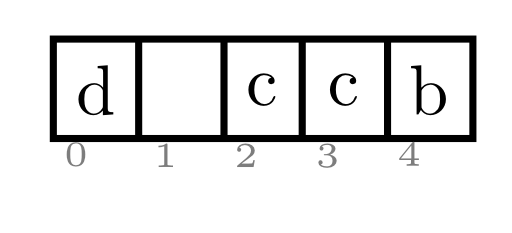
\includegraphics[height=30mm]{array.pdf}
    \begin{itemize}
        \item Indices: 0, 1, 2, 3, 4
        \item Länge des Arrays: 5
        \item Erstes Element: d
    \end{itemize}
\end{frame}

\subsection{Minimalbeispiele}
\begin{frame}{Minimalbeispiele}
Deklarieren:
    \inputminted[linenos=false, numbersep=5pt, tabsize=4,firstline=1, lastline=1, fontsize=\small]{java}{singleLines.java}
\vspace{5 mm}
Deklarieren und instanziieren:
    \inputminted[linenos=false, numbersep=5pt, tabsize=4,firstline=2, lastline=2, fontsize=\small]{java}{singleLines.java}
\vspace{5 mm}
Deklarieren und initialisieren:
    \inputminted[linenos=false, numbersep=5pt, tabsize=4,firstline=3, lastline=4, fontsize=\small]{java}{singleLines.java}
\end{frame}

\subsection{Konvention}
\begin{frame}{Konvention}
    \begin{itemize}
        \item[(A)] Geht, soll man aber nicht machen:
                   \inputminted[linenos=false, numbersep=5pt, tabsize=4,firstline=6, lastline=6, fontsize=\small]{java}{singleLines.java}
        \item[(B)] So ist es gut:
                   \inputminted[linenos=false, numbersep=5pt, tabsize=4,firstline=5, lastline=5, fontsize=\small]{java}{singleLines.java}
    \end{itemize}

    \only<2->{
        Warum ist Variante (B) besser?
        \begin{itemize}
            \item<3-> Der Entwicker kann sofort den Typen sehen
            \item<4-> \href{http://stackoverflow.com/q/13175193/562769}{Konvention}
        \end{itemize}
    }
\end{frame}

\subsection{Ressourcen}
\begin{frame}{Ressourcen}
  \begin{itemize}
    \item \href{http://docs.oracle.com/javase/specs/jls/se7/jls7.pdf}{JLS 7}: Ab S. 291
    \item \href{http://docs.oracle.com/javase/7/docs/api/java/util/Arrays.html}{Java 7 API}
    \item \href{http://docs.oracle.com/javase/tutorial/java/nutsandbolts/arrays.html}{Java Tutorial}
  \end{itemize}
\end{frame}

\section{Random Style Guide}
\subsection{Antipattern: Yoda-Conditions}
\begin{frame}{Antipattern: Yoda-Conditions}
    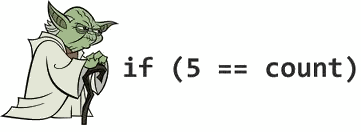
\includegraphics[width=60mm]{yoda-condition.png}\\
    \begin{quote}
        Using \myCode{if(constant == variable)} instead of
        \myCode{if(variable == constant)}, like \myCode{if(4 == foo)}.
        Because it's like saying ``if blue is the sky'' or ``if tall
        is the man''.
    \end{quote}
    Source: \href{http://www.codinghorror.com/blog/2012/07/new-programming-jargon.html}{codinghorror.com}\\

    Bitte nicht machen!
\end{frame}

\subsection{Deklarationen}
\begin{frame}{Deklarationen}
    \begin{itemize}
        \item 1 $\frac{\text{Deklaration}}{\text{Zeile}}$\\
              \vspace{4mm}
              Nicht so:
              \inputminted[linenos=true, numbersep=5pt, tabsize=4, fontsize=\small, firstline=19, lastline=19]{java}{JavaDoc.java}
              \vspace{4mm}
              Sondern so:
              \inputminted[linenos=true, numbersep=5pt, tabsize=4, fontsize=\small, firstline=21, lastline=22]{java}{JavaDoc.java}
        \item Variablen immer dort initialisieren, wo sie deklariert werden\\
              Ausnahme: Initialisierungswert ist von vorherigen Berechnungen abhängig
    \end{itemize}
\end{frame}

\subsection{Antipattern: Stringly Typed}
\begin{frame}{Antipattern: Stringly Typed}
\begin{wrapfigure}{r}{3.1cm}
    
\includegraphics[width=3cm]{stringly-typed.jpg}
\end{wrapfigure}

Used to describe an implementation that \\
needlessly relies on strings.\\
\vspace{2cm}
Excessively stringly typed code is usually\\
a pain to understand and detonates at \\
runtime with errors that the compiler would \\
normally find.

Source: \href{http://www.codinghorror.com/blog/2012/07/new-programming-jargon.html}{codinghorror.com}
\end{frame}

\section{Getter/Setter}
\subsection{Allgemeines}
\begin{frame}{Allgemeines}
    Getter und Setter sind \dots
    \begin{itemize}[<+->]
        \item \dots Methoden
        \item \dots ein "`Interface"'
        \item \dots \href{http://de.wikipedia.org/wiki/Zugriffsfunktion}{Zugriffsfunktionen} zur Abfrage und Änderung
    \end{itemize}
\end{frame}

\subsection{Warum Getter/Setter?}
\begin{frame}{Warum Getter/Setter?}
    Vorteile von Getter und Setter-Methoden sind \dots
    \begin{itemize}[<+->]
        \item \dots (später auftretende) Nebenbedingungen beim get / set
        \item \dots Validierung bei set
        \item \dots Verbergen der Implementierung $\rightarrow$ Geheimnisprinzip
    \end{itemize}
\end{frame}

\subsection{Modifikatoren}
\begin{frame}{Modifikatoren}
  \begin{block}{Zugriffsmodifikatoren}
    Mit Hilfe von \textbf{Zugriffsmodifikatoren} (access modifiers) lassen sich die
    \textbf{Sichtbarkeiten} von Programmteilen regeln:
    \begin{itemize}
        \item \textbf{public} Element: Element ist für alle Klassen sichtbar
        \item<2-> \textbf{private} Element: Element ist nur innerhalb seiner Klasse sichtbar
        \item<3-> \textbf{protected} Element: Element ist nur innerhalb seiner Klasse, deren
              Subklassen und allen Klassen im selben Paket sichtbar
              $\rightarrow$ später mehr dazu
        \item<4-> \textbf{kein Modifier}: Element ist nur innerhalb seiner Klasse und der
              Klassen im selben Paket sichtbar
              $\rightarrow$ hier nicht so wichtig
    \end{itemize}
  \end{block}
\only<5->{
  Ab nun:
  \begin{itemize}
    \item Attribute sind (fast) immer private
    \item Methoden können auch private sein
  \end{itemize}
}
\end{frame}

\subsection{Modifikatoren: Beispiel}
\begin{frame}{Modifikatoren: Beispiel}
  \inputminted[linenos=true, numbersep=5pt, tabsize=4, fontsize=\tiny, frame=lines, label=Student.java, firstline=1, lastline=10]{java}{Visibility.java}
  \inputminted[linenos=true, numbersep=5pt, tabsize=4, fontsize=\tiny, frame=lines, label=Main.java, firstline=12, lastline=19]{java}{Visibility.java}
\end{frame}

\subsection{Modifikatoren: Beispiel}
\begin{frame}{Modifikatoren: Beispiel}
  \begin{alertblock}{Neues Problem}
    Jetzt können wir Namen, Semester und Matrikelnummer von außen gar nicht mehr
    auslesen!
  \end{alertblock}
  \only<2->{
    \begin{block}{Auch hierzu gibt es aber eine Lösung:}
        Mit \textbf{getter-Methoden} kann man den Lesezugriff auf Attribute
        wieder erlauben.
    \end{block}
  }
\end{frame}

\subsection{Modifikatoren: Beispiel}
\begin{frame}{Modifikatoren: Beispiel}
  \inputminted[linenos=true, numbersep=5pt, tabsize=4, fontsize=\tiny, frame=lines, label=Student.java, firstline=21, lastline=30]{java}{Visibility.java}
  \inputminted[linenos=true, numbersep=5pt, tabsize=4, fontsize=\tiny, frame=lines, label=Student.java, firstline=32, lastline=39]{java}{Visibility.java}
\end{frame}

\subsection{Eclipse-Tipp}
\begin{frame}{Eclipse-Tipp}
    \menu{Source > Generate Getters and Setters\dots}\\
    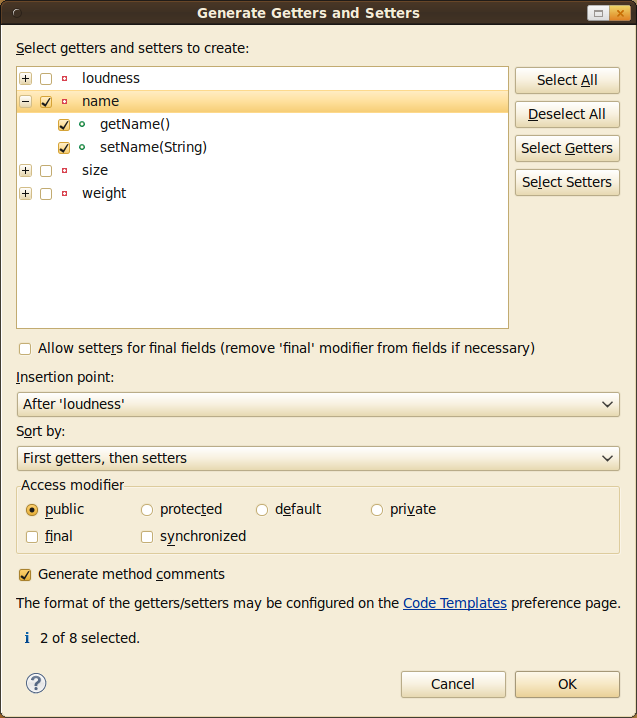
\includegraphics[width=62mm]{eclipse-getter-setter.png}
\end{frame}

\section{Konventionen}
\subsection{Kommentare}
\begin{frame}{Kommentare}
    Typen:
    \begin{itemize}
        \item Implementierungskommentare: \item \myCode{/* blah */} und \myCode{// blah}
        \item Dokumentationskommentare: \myCode{/** blah */}
    \end{itemize}

    \begin{quote}
        Comments should not be enclosed in large boxes drawn with asterisks or other characters.
        Comments should never include special characters such as form-feed and backspace.
    \end{quote}
    Source: \href{http://www.oracle.com/technetwork/java/codeconventions-150003.pdf}{Java Code Conventions}, S. 7 - 9
\end{frame}

\subsection{JavaDoc: Verwendung}
\begin{frame}{JavaDoc: Verwendung}
  Soll fast überall benutzt werden:
  \begin{itemize}
    \item Über jeder Klasse
    \item Über jedem Attribut
    \item Über jeder Methode (mit Annotations)
  \end{itemize}
\end{frame}

\subsection{JavaDoc: Annotations}
\begin{frame}{JavaDoc: Annotations}
  Es gibt folgende Annotations
  \begin{itemize}
    \item \myCode{@param}: Für die Parameter aller Methoden
    \item \myCode{@return}: Für den Rückgabewert vom Methoden
    \item \myCode{@author}: Nur für \myCode{class} und \myCode{interface}, erforderlich
  \end{itemize}
  \vspace{0.5cm}
  Weitere Annotations:
  \begin{itemize}
    \item \myCode{@throws}: Angabe möglicher Fehlermeldungen
  \end{itemize}
\end{frame}

\subsection{JavaDoc: Negativ-Beispiel}
\begin{frame}{JavaDoc: Negativ-Beispiel}
  \inputminted[linenos=true, numbersep=5pt, tabsize=4, fontsize=\small, firstline=1, lastline=6]{java}{JavaDoc.java}

  \begin{itemize}
    \item Was ist hier schlecht?
    \item Wie könnte man es verbessern?
  \end{itemize}
\end{frame}

\subsection{JavaDoc: Positiv-Beispiel}
\begin{frame}{JavaDoc: Positiv-Beispiel}
  \inputminted[linenos=true, numbersep=5pt, tabsize=4, fontsize=\small, firstline=9, lastline=16]{java}{JavaDoc.java}
\end{frame}

\section{Kontrollstrukturen}
\subsection{if-Abfragen}
\begin{frame}{if-Abfragen}
  \inputminted[linenos=true, numbersep=5pt, tabsize=4, fontsize=\small, firstline=1, lastline=5]{java}{Kontrollstrukturen.java}

  KEINE Schleife! $\rightarrow$ \href{http://if-schleife.de/}{if-schleife.de}
\end{frame}

\subsection{if-Abfragen: else if}
\begin{frame}{if-Abfragen: else if}
  \inputminted[linenos=true, numbersep=5pt, tabsize=4, fontsize=\small, firstline=7, lastline=13]{java}{Kontrollstrukturen.java}
\end{frame}

\subsection{if-Abfragen: Quiz}
\begin{frame}{if-Abfragen: Quiz}
  \inputminted[linenos=true, numbersep=5pt, tabsize=4, fontsize=\small, frame=lines]{java}{QuizIf.java}
\end{frame}

\subsection{for-Schleifen}
\begin{frame}{for-Schleifen}
  \begin{itemize}
    \item Syntax: \myCode{for ([INITIALISIERUNG; BEDINGUNG; UPDATE]) \{ \dots \}}
  \end{itemize}

  \inputminted[linenos=true, numbersep=5pt, tabsize=4, fontsize=\small, firstline=39, lastline=41]{java}{Kontrollstrukturen.java}
\end{frame}

\subsection{while-Schleifen}
\begin{frame}{while-Schleifen}
  \begin{itemize}
    \item Syntax: \myCode{while ([BEDINGUNG]) \{ \dots \}}
  \end{itemize}

  \inputminted[linenos=true, numbersep=5pt, tabsize=4, fontsize=\small, firstline=35, lastline=37]{java}{Kontrollstrukturen.java}
\end{frame}

\subsection{do-while-Schleifen}
\begin{frame}{do-while-Schleifen}
  \begin{itemize}
    \item Syntax: \myCode{do \{ \dots \} while ([BEDINGUNG]);}
    \item Wo ist der Unterschied zu \myCode{while}?
  \end{itemize}

  \inputminted[linenos=true, numbersep=5pt, tabsize=4, fontsize=\small, firstline=43, lastline=49]{java}{Kontrollstrukturen.java}
\end{frame}

\subsection{Switch-Anweisung}
\begin{frame}{Switch-Anweisung}
  \inputminted[linenos=true, numbersep=5pt, tabsize=4, fontsize=\tiny, frame=lines, firstline=15, lastline=33, label=World.java]{java}{Kontrollstrukturen.java}
\end{frame}

\section{Praxis}
\subsection{Praxis}
\begin{frame}{Praxis}
  Falls noch Zeit bleibt \dots
\end{frame}

\section{Abspann}
\subsection{Kommende Tutorien}
\begin{frame}{Kommende Tutorien}
  \begin{itemize}
    \item[11.] 05.11.2012
    \item[10.] 12.11.2012
    \item[9.] 19.11.2012
    \item[8.] 26.11.2012
    \item[7.] 03.12.2012
    \item[6.] 10.12.2012
    \item[5.] 17.12.2012: Video "`Library"' zeigen
    \item[-] 24.12.2012: Heiligabend - \href{http://www.fmc.uni-karlsruhe.de/faq/wann-sind-die-weihnachtsferien}{Kein Tutorium}
    \item[-] 31.12.2012: Silvester - Kein Tutorium
    \item[4.] 07.01.2013
    \item[3.] 14.01.2013
    \item[2.] 21.01.2013
    \item[1.] 28.01.2013
    \item[0.] 04.02.2013
    \item[-] 10.02.2013: Ende der Vorlesungszeit des WS 2012/2013 (\href{http://www.kit.edu/studieren/2873.php}{Quelle})
  \end{itemize}
\end{frame}

\framedgraphic{Vielen Dank für eure Aufmerksamkeit!}{../images/geekandpoke-2010-10.jpg}

\end{document}
